%
%   section 4
%
%   2018/11/26

\documentclass[11pt,b5paper,papersize,dvipdfmx]{jsbook}

\usepackage{vuccaken}
\usepackage{vuccaken2018}
\usepackage{12nkym}


\begin{document}
% \tableofcontents % 目次出力
% \clearpage


% - - - - - - - - - - - - - - - - -
\section{リーマン予想}
\label{sec:4}
% - - - - - - - - - - - - - - - - -

最後にリーマン予想の話をしよう。だがその前にゼータ関数についてもう少し詳しくなっておこう。
まず、ゼータ関数の解析接続を別の方法(積分表示)で与える。この表示による副産物として、$s$が負の整数のときの$\zeta(s)$の値をベルヌーイ数を用いて簡単に計算できるようになる。ここでゼータ関数の自明な零点についても説明する。また、$s$が正の偶数であるときの$\zeta(s)$の値もベルヌーイ数を用いて計算できることを示す。\par
次に$0\le \Re(s) \le 1$を除いた領域では$\zeta(s)$は零点を持たないことを示し、$\zeta(s)$非自明な零点について説明する。ただしこの辺で私が力尽きてしまったので、証明はいくつか省略している。\par
以上のことを踏まえ、ここでようやくリーマン予想について説明する。素数定理というものを見ながら、リーマン予想がどういう意味を持つのかについて考えていく。\par
最後に、Fortranを用いて$\Re(s)=\frac12$上にある$\zeta(s)$の零点を数値計算で求めてみたので、その結果を載せておく。

\clearpage
% - - - - - - - - - - - - - - - - -
\subsection{ガンマ関数$\Gamma(s)$}
% - - - - - - - - - - - - - - - - -
まずはゼータ関数の積分表示に必要なガンマ関数を定義する。
\begin{thm}{定義(ガンマ関数)}
  複素数$s$について、積分で定義された関数
  \begin{align}
    \Gamma(s) := \int_0^\infty e^{-x} x^{s-1} \dd{x}
    \label{eq:Gamma-def}
  \end{align}
  は、$\Re(s) > 0$で一様に絶対収束し、正則関数となる。$\Gamma(s)$はガンマ関数と呼ばれる。
\end{thm}
\begin{prf}
  右辺の広義積分が$\Re(s)>0$で絶対収束することを示す。
  $x>0$と任意の$0 \le m \in \mathbb{Z}$に対し
  \begin{align*}
    e^x &= \sum_{n=0}^\infty \frac{x^n}{n!}
    = 1 + x + \frac{x^2}{2} + \cdots + \frac{x^m}{m!} + \cdots
    \ge \frac{x^m}{m!}
  \end{align*}
  であるから、$ e^{-x} \le m!\, x^{-m} $
  であり、$s\equiv \sigma + it$とおくと、$0<\sigma<m$なる任意の$\sigma,m$に対し
  \begin{align*}
    \int_0^\infty |e^{-x} x^{s-1}| \dd{x}
    &= \int_0^\infty e^{-x} x^{\sigma-1} \dd{x}\\
    &= \int_0^1 e^{-x} x^{\sigma-1} \dd{x}
      + \int_1^\infty e^{-x} x^{\sigma-1} \dd{x}\\
    &\le \int_0^1 x^{\sigma-1} \dd{x} + m! \int_1^\infty x^{\sigma-m-1} \dd{x}\\
    &= \qty[\frac{x^\sigma}{\sigma}]_0^1 + m! \qty[\frac{x^{\sigma-m}}{\sigma-m}]_1^\infty\\
    &= \frac1\sigma + \frac{m!}{m-\sigma}
  \end{align*}
  となるので、積分は収束する。また
  \begin{align*}
    \Gamma_n(s) := \int_{\frac1n}^n e^{-t} t^{s-1} \dd{t}
    \qquad (n=1,2,3,\cdots)
  \end{align*}
  とおくと、各$\Gamma_n(s)$は$\Re(s)>0$で正則である。
  さらに、$0<a<b$とするとき、$a \le \Re(s) \le b$ならば
  % \begin{align*}
  %   \qty| \Gamma_n(s) - \Gamma(s) |
  %   &= \qty| \int_{\frac1n}^n e^{-t} t^{s-1} \dd{t} - \int_0^\infty e^{-t} t^{s-1} \dd{t}|\\
  %   &= \qty| \int_{\frac1n}^n e^{-t} t^{s-1} \dd{t} - \qty\bigg( \int_0^{\frac1n} e^{-t} t^{s-1} \dd{t} + \int_{\frac1n}^n e^{-t} t^{s-1} \dd{t} + \int_n^\infty e^{-t} t^{s-1} \dd{t} ) |\\
  %   &= \qty| \int_0^{\frac1n} e^{-t} t^{s-1} \dd{t} + \int_n^\infty e^{-t} t^{s-1} \dd{t} |
  % \end{align*}
  \begin{align*}
    \Gamma(s) - \Gamma_n(s)
    &= \qty\bigg(\int_0^\infty - \int_{\frac1n}^n)\, e^{-t} t^{s-1} \dd{t}\\
    &= \qty\bigg(\int_0^{\frac1n} + \int_{\frac1n}^n + \int_n^\infty - \int_{\frac1n}^n)\, e^{-t} t^{s-1} \dd{t}\\
    &= \qty\bigg(\int_0^{\frac1n} + \int_n^\infty)\, e^{-t} t^{s-1} \dd{t}\\
  \end{align*}
  であるから
  \begin{align*}
    \qty| \Gamma(s) - \Gamma_n(s) |
    &= \qty| \int_0^{\frac1n} e^{-t} t^{s-1} \dd{t} + \int_n^\infty e^{-t} t^{s-1} \dd{t} |\\
    &\le \qty|\int_0^{\frac1n} e^{-t} t^{s-1} \dd{t}| + \qty|\int_n^\infty e^{-t} t^{s-1} \dd{t}|\\
    &\le \int_0^{\frac1n} \qty|e^{-t} t^{s-1}| \dd{t} + \int_n^\infty \qty|e^{-t} t^{s-1}| \dd{t}\\
    &= \int_0^{\frac1n} e^{-t} t^{s-1} \dd{t} + \int_n^\infty e^{-t} t^{s-1} \dd{t}\\
    &\le \int_0^{\frac1n} e^{-t} t^{a-1} \dd{t} + \int_n^\infty e^{-t} t^{b-1} \dd{t}.
  \end{align*}
  ゆえに、$\Re(s)>0$で$\Gamma_n(s)$は$\Gamma(s)$に一様収束する。
  よって、$\Re(s)>0$で$\Gamma(s)$は正則である。
\end{prf}

%
以下に示す性質から、ガンマ関数とは自然数$n$の階乗$n!$を複素数の範囲にまで拡張したのものであると理解できる。
\begin{thm}{定理(ガンマ関数の性質)}
  $\Re(s) > 0$のとき、関係式
  \begin{align}
    \Gamma(s+1) = s\Gamma(s)
    % \label{eq:Gamma-1}
  \end{align}
  が成り立つ。特に$s$が自然数$n$のとき
  \begin{align}
    \Gamma(n) = (n-1)!
  \end{align}
  となる。
\end{thm}
\begin{prf}
  $\Re(s) > 0$であると仮定すると、部分積分より
  \begin{align*}
    \Gamma(s+1) &= \int_0^\infty e^{-x} x^s \dd{x}\\
    &= \qty[ (-e^{-x}) x^s ]_0^\infty
      - \int_0^\infty (-e^{-x}) s x^{s-1} \dd{x}\\
    &= 0 + s \int_0^\infty e^{-x} x^{s-1} \dd{x}\\
    &= s\Gamma(s).
  \end{align*}
  また、$ \Gamma(1) = \int_0^\infty e^{-x} \dd{x} = 1 $であるから、
  自然数$n$について$ \Gamma(n) =(n-1)! $が言える。
\end{prf}

%
先ほど求めた関係式を用いて、ガンマ関数を複素数全体へ解析接続する。
\begin{thm}{定理(ガンマ関数の解析接続)}
  ガンマ関数は複素数全体に解析接続される。
  ガンマ関数は零点を持たず、$s=0,-1,-2,\cdots$にのみ1位の極を持つ。
  これらの極を除いた複素数全体で正則関数となる。
\end{thm}
\begin{prf}
  $0 < \Re(s) < 1$における$\Gamma(s)$の値から、関係式
  \begin{align*}
    \Gamma(s) = \frac{\Gamma(s+1)}{s}
  \end{align*}
  によって、$\Gamma(s)$の定義域を$\Re(s) > -1$にまで延長できる。
  これを繰り返し行うことにより、$\Re(s) > -2, \Re(s) > -3, \cdots$と次々に延長でき、$\Gamma(s)$は複素数全体へ解析接続される。\par
  また、$s=0,-1,-2,\cdots$にのみ極を持ち、それらが全て1位の極であることは、上の関係式によりすぐにわかる。
  零点を持たないことは、後述の相反公式からわかる。
\end{prf}

%
次に、$\Gamma(s)$の相反公式というものを示す。この式によって$\Gamma(s)$が零点を持たないことがわかる。つまり$\dfrac1{\Gamma(s)}$は複素平面全体で正則関数となる。\par
$\Gamma(s)$の相反公式を示す準備として、まずは次の定積分の値を求めておこう。
%
\begin{thm}{定理}
  $0 < \alpha < 1$のとき
  \begin{align}
    \int_{-\infty}^\infty \frac{e^{\alpha x}}{1+e^x}\dd{x}
    = \frac{\pi}{\sin \pi\alpha}
    \label{eq:int-sin}
  \end{align}
  が成り立つ。
\end{thm}
%
\clearpage
%
\begin{prf}
  %
  \begin{figure}[H]
    \centering
    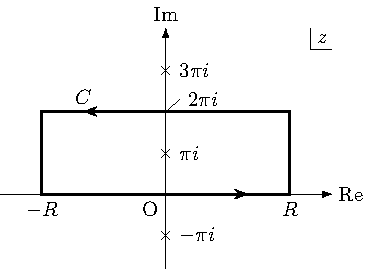
\includegraphics{nkym/fig/pi-sin}
    \caption{積分路$C$と$f(z)$の極}
    \label{fig:pi-sin}
  \end{figure}
  %
  $f(z):=\dfrac{e^{\alpha z}}{1+e^z} \,\, (0<\alpha<1)$とし、
  図\ref{fig:pi-sin}のような経路$C$に沿った積分の値を、留数定理を用いた方法と、直接積分を実行する方法の2通りの方法で求める。\par
  まず、$f(z)$は極を$z=(2n+1)\pi i \,\, (n\in\mathbb{Z})$に持ち、それらはすべて単純極である。よって経路$C$内の極は$z=\pi i$のみであり、そこでの留数は
  \begin{align*}
    \Res_{z=\pi i}[f]
    &= \lim_{z\to\pi i} (z-\pi i) \frac{e^{\alpha z}}{1+e^z}\\
    &= \lim_{\zeta\to 0} \zeta \cdot \frac{e^{\alpha(\zeta+\pi i)}}{1+e^{\zeta+\pi i}} \quad (\because \zeta := z - \pi i)\\
    &= e^{\pi i \alpha}\cdot \lim_{\zeta\to 0} \zeta \cdot \frac{e^{\alpha\zeta}}{1-e^\zeta} \quad (\because e^{\pi i} = -1)\\
    &= e^{\pi i \alpha}\cdot \lim_{\zeta\to 0} \frac{\zeta}{1-e^\zeta}\\
    &= e^{\pi i \alpha}\cdot \lim_{\zeta\to 0} \frac{\zeta}{1-\qty{1+\zeta+\order{\zeta^2}}}\\
    &= e^{\pi i \alpha}\cdot \lim_{\zeta\to 0} \frac1{-1+\order{\zeta}}\\
    &= -e^{\pi i \alpha}
  \end{align*}
  であるから、留数定理より
  \begin{align*}
    \oint_C f(z) \dd{z} = 2\pi i \cdot \Res_{z=\pi i}[f]
    = -2\pi i e^{\pi i \alpha}
  \end{align*}
  となる。$R\to\infty$としてもこの値は変わらない。\par
  一方、経路$C$を各辺ごとに分解すると
  \begin{align*}
    \oint_C f(z) \dd{z} 
    &= \int_{-R}^R \frac{e^{\alpha x}}{1+e^x} \dd{x}
      + \int_0^{2\pi} \frac{e^{\alpha(R+iy)}}{1+e^{R+iy}} \,i\dd{y}\\
      &\qquad\quad + \int_R^{-R} \frac{e^{\alpha(x+2\pi i)}}{1+e^{x+2\pi i}} \dd{x}
      + \int_{2\pi}^0 \frac{e^{\alpha(-R+iy)}}{1+e^{-R+iy}} \,i\dd{y}.
  \end{align*}
  ここで
  \begin{align*}
    |\text{第2項}|
    &= \qty|\int_0^{2\pi} \frac{e^{\alpha(R+iy)}}{1+e^{R+iy}} \,i\dd{y}|
    \le \int_0^{2\pi} \qty|\frac{e^{\alpha(R+iy)}}{1+e^{R+iy}}| \dd{y}\\
    &= \int_0^{2\pi} \frac{|e^{\alpha R}||e^{iy}|}{|1+e^R e^{iy}|} \dd{y}
    = \int_0^{2\pi} \frac{e^{\alpha R}} {|1+e^R e^{iy}|} \dd{y}\\
    &\le \int_0^{2\pi} \frac{e^{\alpha R}} {|e^R e^{iy}|-1} \dd{y}
    = \int_0^{2\pi} \frac{e^{\alpha R}} {e^R-1} \dd{y}\\
    &= 2\pi \cdot \frac{e^{\alpha R}} {e^R-1}
    = 2\pi \cdot \frac{e^{-(1-\alpha) R}} {1-e^{-R}}\\
    &\xrightarrow{R\to\infty} 2\pi \cdot \frac{0}{1-0} = 0,
  \end{align*}
  \begin{align*}
    |\text{第4項}|
    &= \qty| \int_{2\pi}^0 \frac{e^{\alpha(-R+iy)}}{1+e^{-R+iy}} \,i\dd{y}|
    \le \int_0^{2\pi} \qty|\frac{e^{\alpha(-R+iy)}}{1+e^{-R+iy}}| \dd{y}\\
    &\le \int_0^{2\pi} \frac{e^{-\alpha R}}{1-e^{-R}} \dd{y}
    = 2\pi \cdot \frac{e^{-\alpha R}}{1-e^{-R}}\\
    &\xrightarrow{R\to\infty} 2\pi \cdot \frac{0}{1-0} = 0,
  \end{align*}
  \begin{align*}
    \text{第3項}
    &= \int_R^{-R} \frac{e^{\alpha(x+2\pi i)}}{1+e^{x+2\pi i}} \dd{x}
    = -\int_{-R}^R \frac{e^{\alpha x} e^{2\pi i\alpha}}{1+e^x e^{2\pi i}} \dd{x}\\
    &= - e^{2\pi i\alpha}\int_{-R}^R \frac{e^{\alpha x}}{1+e^x} \dd{x}
  \end{align*}
  となるので
  \begin{align*}
    \oint_C f(z) \dd{z}
    &= \int_{-\infty}^\infty \frac{e^{\alpha x}}{1+e^x} \dd{x}
    + 0 + 0 - e^{2\pi i\alpha}\int_{-\infty}^\infty \frac{e^{\alpha x}}{1+e^x} \dd{x}\\
    &= \qty(1-e^{2\pi i\alpha}) \int_{-\infty}^\infty \frac{e^{\alpha x}}{1+e^x} \dd{x}.
  \end{align*}\par
  よって、これら2通りの方法で求めた積分値が等しいので
  \begin{align*}
    \qty(1-e^{2\pi i\alpha}) \int_{-\infty}^\infty \frac{e^{\alpha x}}{1+e^x} \dd{x}
    = -2\pi i e^{\pi i \alpha}.
  \end{align*}
  $1-e^{2\pi i\alpha} \ne 0$であるから
  \begin{align*}
    \int_{-\infty}^\infty \frac{e^{\alpha x}}{1+e^x} \dd{x}
    &= \frac{2\pi i e^{\pi i \alpha}}{e^{2\pi i\alpha}-1}\\
    &= \frac{2\pi i}{e^{\pi i\alpha}-e^{-\pi i\alpha}}\\
    &= \frac{\pi}{\sin \pi \alpha}
      \quad \qty\Big(\because \sin z = \frac{e^{iz}-e^{-iz}}{2i} )
  \end{align*}
  となる。
\end{prf}

%
相反公式の証明で実際に用いるのは、上の式で$t:=e^x$と変数変換した次の式である。
\begin{thm}{定理}
  $0<\alpha<1$のとき
  \begin{align}
    \int_0^\infty \frac{x^{\alpha-1}}{1+x} \dd{x}
    = \frac{\pi}{\sin \pi \alpha}
  \end{align}
  が成り立つ。
\end{thm}
\begin{prf}
  (\ref{eq:int-sin})において$t := e^x$と変数変換すれば
  \begin{align*}
    \frac{\pi}{\sin \pi \alpha}
    &= \int_{-\infty}^\infty \frac{e^{\alpha x}}{1+e^x}\dd{x}
    = \int_0^\infty \frac{t^\alpha}{1+t} \cdot \frac{\dd{t}}{t}
      \quad (\because t := e^x)\\
    &= \int_0^\infty \frac{t^{\alpha-1}}{1+t} \dd{t}.
  \end{align*}
\end{prf}

ここでさらにベータ関数と呼ばれるものを定義する。下記の関係式からもわかるように、ベータ関数はガンマ関数と深く結びついている。
\begin{thm}{定義&命題}
  $\Re(p),\Re(q) > 0$であるような複素数$p,q$について、ベータ関数を
  \begin{align}
    B(p,q) := \int_0^1 x^{p-1} (1-x)^{q-1} \dd{x}
  \end{align}
  と定義すると、以下の関係式が成り立つ。
  \begin{align}
    B(p,q) &= \int_0^\infty \frac{x^{p-1}}{(1+x)^{p+q}} \dd{x},\quad
    B(p,q) = \frac{\Gamma(p) \Gamma(q)}{\Gamma(p+q)}
  \end{align}
\end{thm}
\begin{prf}
  まず、ベータ関数の定義式において、変数変換$x =: \dfrac{t}{1+t}$を行うことで
  \begin{align*}
    B(p,q) &= \int_0^\infty \qty(\frac{t}{1+t})^{p-1} \qty(1-\frac{t}{1+t})^{q-1} \frac{\dd{t}}{(1+t)^2} \\
    &= \int_0^\infty \frac{t^{p-1}}{(1+t)^{p+q}} \dd{t}
  \end{align*}
  が得られる。\par
  次に、ガンマ関数の定義式から
  \begin{align*}
    \Gamma(p)\Gamma(q)
    &= \qty( \int_0^\infty e^{-x} x^{p-1} \dd{x} )
      \qty( \int_0^\infty e^{-y} y^{q-1} \dd{y} )
  \end{align*}
  であり、$x=:X^2,\, y=:Y^2$と変数変換を行うと
  \begin{align*}
    \Gamma(p)\Gamma(q)
    &= \qty( \int_0^\infty e^{-X^2} X^{2(p-1)} \cdot 2X\dd X )
      \qty( \int_0^\infty e^{-Y^2} Y^{2(q-1)} \cdot 2Y\dd Y )\\
    &= 4\int_0^\infty \dd{X} \int_0^\infty \dd{Y}
      e^{-(X^2+Y^2)} X^{2p-1} Y^{2q-1}.
  \end{align*}
  ここで、$X=:r\cos\theta,\, Y=:r\sin\theta$と変数変換を行うと
  \begin{align*}
    \Gamma(p)\Gamma(q)
    &= 4\int_0^\infty \dd{r} \int_0^\frac{\pi}{2} \dd{\theta}
      r e^{-r^2} (r\cos\theta)^{2p-1} (r\sin\theta)^{2q-1}\\
    &= \qty\bigg( 2\int_0^\frac{\pi}{2} \cos^{2p-1}\theta \sin^{2q-1}\theta \dd{\theta})
      \qty( 2\int_0^\infty e^{r^2} r^{2p+2q-1} \dd{r} ).
  \end{align*}
  後半部分は、$R:= r^2$と変数変換すれば$\dd{R} = 2r\dd{r}$であるから
  \begin{align*}
    2\int_0^\infty e^{r^2} r^{2p+2q-1} \dd{r}
    &= \int_0^\infty e^R R^{p+q-1} \dd{R} = \Gamma(p+q)
  \end{align*}
  となる。前半部分は、ベータ関数の定義式において$x=:\sin^2\theta$と変数変換すれば、$\dd{x} = 2\sin\theta\cos\theta\dd{\theta}$であるから
  \begin{align*}
    B(p,q) &= \int_0^\frac{\pi}{2} \sin^{2(p-1)}\theta (1-\sin^2\theta)^{q-1} \cdot 2\sin\theta\cos\theta\dd{\theta}\\
    &= 2\int_0^\frac{\pi}{2} \sin^{2q-1}\theta \cos^{2p-1}\theta \dd{\theta}
  \end{align*}
  となる。よって
  \begin{align*}
    \Gamma(p) \Gamma(q) = B(p,q) \Gamma(p+q).
  \end{align*}
\end{prf}


\begin{thm}{定理(相反公式)}
  \begin{align}
    \Gamma(s)\Gamma(1-s) = \frac{\pi}{\sin \pi s}
    \quad (s\in\mathbb{C} \setminus \mathbb{Z})
    \label{eq:gamma-souhan}
  \end{align}
\end{thm}
\begin{prf}
  $0<\alpha<1$のとき
  \begin{align*}
    \Gamma(\alpha)\Gamma(1-\alpha) = B(\alpha,1-\alpha)
    = \int_0^\infty \frac{x^{\alpha-1}}{1+x} \dd{x}
    = \frac{\pi}{\sin \pi \alpha}
  \end{align*}
  であるから、一致の定理より
  \begin{align*}
    \Gamma(s)\Gamma(1-s) = \frac{\pi}{\sin \pi s}
    \quad (s\in\mathbb{C} \setminus \mathbb{Z})
  \end{align*}
  となる。
\end{prf}
\begin{remark}
  前にも書いたように、この相反公式(\ref{eq:gamma-souhan})から$\Gamma(s)$は零点を持たないことがわかる。さらに$\dfrac1{\Gamma(s)}$は複素平面全体で正則な関数であり、$s=-k\,\,(k=1,2,3,\cdots)$に1位の零点を持つ。
  \begin{align}
    \frac1{\Gamma(-k)} = 0 \quad (k= 1,2,3,\cdots).
  \end{align}
\end{remark}

また、(\ref{eq:Gamma-1})の代わりに相反公式(\ref{eq:gamma-souhan})を用いることでもガンマ関数$\Gamma(s)$を解析接続することができる。すなわち、$\Re(s)\le0$のとき
\begin{align}
  \Gamma(s) = \frac{\pi}{\Gamma(1-s) \sin \pi s}
  % \label{eq:gamma-setuzoku-sohan}
\end{align}
によって$\Gamma(s)$を定義してもかまわない。$s=0,-1,-2,\cdots$に極を持つこともすぐにわかる。こちらの方法で$\Gamma(s)$を解析接続する方が、一発で$\Gamma(s)$の値が求まるので実用的である。

% - - - - - - - - - - - - - - - - -
\subsection{積分表示による$\zeta(s)$の解析接続}
% - - - - - - - - - - - - - - - - -

前節で定義したガンマ関数$\Gamma(s)$を用いて、第\ref{sec:zeta}節とは異なった方法で、再びゼータ関数$\zeta(s)$を解析接続する。この解析接続の副産物として、$s$が負の整数のときの$\zeta(s)$の値を求める一般公式を得ることができる。\par
それではまず、$B_n$はベルヌーイ数と呼ばれる有理数を定義するところから始めよう。

%
\begin{thm}{定義(ベルヌーイ数)}
  ベルヌーイ数$B_n$を以下のマクローリン展開の展開係数として定義する。
  \begin{align}
    \frac{x}{e^x - 1} = \sum_{n=0}^\infty \frac{B_n}{n!}x^n.
    \label{eq:berunui}
  \end{align}
\end{thm}

上の定義からベルヌーイ数を計算するのは容易ではなく
\footnote{
  $ \displaystyle B_n = \eval{ \dv[n]{x} \qty( \frac{x}{e^x - 1} ) }_{x=0} $
  で計算できるが、かなり面倒臭い。
} 、
以下の漸化式が有用である。

\begin{thm}{定理(ベルヌーイ数の漸化式)}
  \begin{align}
    B_0 = 1,\quad B_n = -\frac{1}{n+1} \sum_{k=0}^{n-1} \binom{n+1}{k}B_k
    \label{eq:B-zenkasiki}
  \end{align}
\end{thm}
%
\begin{remark}
  この漸化式から、ベルヌーイ数$B_n$は有理数であることがわかる。
\end{remark}
%
\begin{prf}
  $f(x) = \dfrac{x}{e^x - 1}$とその逆数をテイラー展開し、それらの積が恒等的に$1$であることからベルヌー数が満たす漸化式を求める。$f(x)$の逆数のテイラー展開は\\
  \begin{align*}
    \frac1{f(x)} &= \frac{e^x-1}{x}
    = \frac1{x} \qty( \sum_{n=0}^\infty \frac{x^n}{n!} - 1 )
    = \frac1{x} \sum_{n=1}^\infty \frac{x^n}{n!}\\
    &= \sum_{n=1}^\infty \frac{x^{n-1}}{n!}
    = \sum_{n=0}^\infty \frac{x^n}{(n+1)!}
  \end{align*}
  であるから
  \begin{align*}
    1 &= f(x) \cdot \frac1{f(x)}
    = \qty( \sum_{i=0}^\infty \frac{B_i}{i!}x^i ) \qty( \sum_{j=0}^\infty \frac{x^j}{(j+1)!} )\\
    &= \sum_{i=0}^\infty \sum_{j=0}^\infty \frac{B_i}{i!(j+1)!} x^{i+j}
  \end{align*}
  ここで、図\ref{fig:naname}のように二重和の取り方を変更する。$i,j$について縦横に足し上げるのではなく、$i+j=:n$を固定し、斜め方向に足し上げていく。
  %
  \begin{figure}[H]
    \centering
    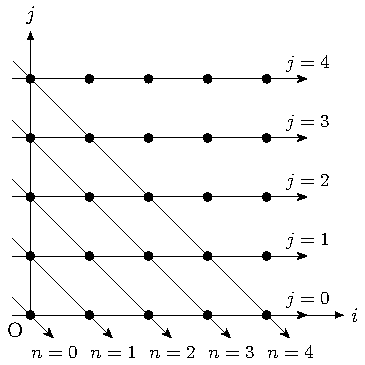
\includegraphics{nkym/fig/naname.pdf}
    \caption{二重和の取り方の変更。}
    \label{fig:naname}
  \end{figure}
  %
  すると
  \begin{align*}
    1 = \sum_{n=0}^\infty \sum_{k=0}^n \frac{B_k}{k!(n-k+1)!} x^n
    \quad (n:=i+j,\, k:=i)
  \end{align*}
  となり、各$x^n$の係数を比較すると
  \begin{align*}
    \begin{cases}
      1 = B_0 \vphantom{\dfrac00} &\quad (n=0),\\
      0 = \displaystyle\sum_{k=0}^n \dfrac{B_k}{k!(n-k+1)!} &\quad (n\ge1)
    \end{cases}
  \end{align*}
  が得られる。第2式は
  \begin{align*}
    0 = \sum_{k=0}^{n-1} \frac{B_k}{k!(n-k+1)!} + \frac{B_n}{n!}
  \end{align*}
  となるので
  \begin{align*}
    B_n &= - n! \sum_{k=0}^{n-1} \frac{B_k}{k!(n-k+1)!}\\
    &= -\frac1{n+1} \sum_{k=0}^{n-1} \frac{(n+1)!}{k!(n-k+1)!} B_k\\
    &= -\frac1{n+1} \sum_{k=0}^{n-1} \binom{n+1}{k} B_k.
  \end{align*}
  よって漸化式(\ref{eq:B-zenkasiki})が得られる。
\end{prf}

\begin{thm}{ベルヌーイ数$B_n$の具体的な値}\par
  %
  \begin{minipage}{0.3\hsize}
    \begin{align*}
      B_0 &= 1,\\
      B_1 &= -\frac12,\\
      B_2 &= \frac16,\\
      B_3 &= 0,\\
      B_4 &= -\frac1{30},
    \end{align*}
  \end{minipage}
  %
  \begin{minipage}{0.3\hsize}
    \begin{align*}
      B_5 &= 0,\\
      B_6 &= \frac1{42},\\
      B_7 &= 0,\\
      B_8 &= -\frac1{30},\\
      B_9 &= 0,
    \end{align*}
  \end{minipage}
  %
  \begin{minipage}{0.3\hsize}
    \begin{align*}
      B_{10} &= \frac5{66},\\
      B_{11} &= 0,\\
      B_{12} &= -\frac{691}{2730},\\
      B_{13} &= 0,\\
      B_{14} &= \frac76.
    \end{align*}
  \end{minipage}
  %
\end{thm}
%
\begin{remark}
  $k$が3以上の奇数のとき$B_k = 0$である。このことは第\ref{sec:zeta-sp}節で示す。
\end{remark}

%
ディリクレ表示で定義されたゼータ関数$\zeta(s)$は、ガンマ関数$\Gamma(s)$を用いて以下のように積分表示できる。
ただし、定義域は相変わらず$\Re(s) > 1$である。
\begin{thm}{定理(リーマンの第一積分表示)}
  \begin{align}
    \zeta(s) = \frac{1}{\Gamma(s)} \int_0^\infty \frac{x^{s-1}}{e^x - 1} \dd{x}
    \qquad (\Re(s) > 1).
  \end{align}
\end{thm}
\begin{prf}
  $x>0$において、等比級数の和の公式より
  \begin{align*}
    \sum_{n=1}^\infty e^{-nx} &\equiv e^{-x} + e^{-2x} + e^{-3x} + \cdots\\
    % &= e^{-x} \,\qty(1 + e^{-x} + e^{-2x} + \cdots)\\
    &= \frac{e^{-x}}{1 - e^{-x}}
    = \frac{1}{e^x - 1}
  \end{align*}
  であることを用いて
  \begin{align*}
    \int_0^\infty \frac{x^{s-1}}{e^x - 1} \dd{x}
    &= \int_0^\infty x^{s-1} \sum_{n=1}^\infty e^{-nx} \dd{x} \\
    &= \sum_{n=1}^\infty \int_0^\infty x^{s-1} e^{-nx} \dd{x} \\
    &= \sum_{n=1}^\infty n^{-s} \int_0^\infty u^{s-1} e^{-u} \dd{u}
    \qquad (u:=nx) \\
    &= \Gamma(s) \sum_{n=1}^\infty n^{-s} 
    = \Gamma(s) \cdot \zeta(s).
  \end{align*}
\end{prf}


%
上の積分表示では$\zeta(s)$の定義域は$\Re(s)>1$のままであるが、次のように積分を分解することで、$\zeta(s)$を$s=1$を除く複素平面全体に解析接続することができる!
\begin{align*}
  \zeta(s) = \frac{1}{\Gamma(s)} \int_0^\infty \frac{x^{s-1}}{e^x - 1} \dd{x}
  = \mathrm{I}(s) + \mathrm{II}_k(s) + \mathrm{III}_k(s).
\end{align*}
ここで
\begin{align*}
  \mathrm{I}(s) &= \frac{1}{\Gamma(s)} \int_1^\infty \frac{x^{s-1}}{e^x - 1} \dd{x},\\
  \mathrm{II}_k(s) &= \frac{1}{\Gamma(s)} \int_0^1 \qty( \frac{1}{e^x - 1}
  - \sum_{\ell = 0}^{k+1} \frac{B_\ell}{\ell !} x^{\ell - 1} ) x^{s-1} \dd{x},\\
  \mathrm{III}_k(s) &= \frac{1}{\Gamma(s)} \int_0^1 \qty( \sum_{\ell = 0}^{k+1} \frac{B_\ell}{\ell !} x^{\ell - 1} ) x^{s-1} \dd{x}
\end{align*}
である。また、$k$は$k \ge 0$を満たす整数とし、$B_\ell$はベルヌーイ数である。\par
このように積分を3つに分割して書くことで、$\Re(s)>1$でしか定義されなかったゼータ関数$\zeta(s)$を、$s=1$の一点を除き、各整数$k$に対し$\Re(s) > -k-1$にまで解析接続できる。
つまり、いくらでも大きな整数$k$を取れば、ゼータ関数$\zeta(s)$は$s=1$を除いた全ての複素数で正則となるように解析接続できる!! そのことを以下で詳しく見てみよう。

%
まず、$\dfrac{1}{\Gamma(s)}$は複素数全体で正則な関数である。
さらに、$\mathrm{I}(s)$の積分は、被積分関数の分母の指数関数の方が収束が速いので、$s$の値に依らず有限値に収束し、$\mathrm{I}(s)$は複素数全体で正則関数となる。\par

%
次に、$\mathrm{II}_k(s)$の被積分関数は、ベルヌーイ数の定義を思い出すと
\begin{align*}
  \qty( \frac{1}{e^x - 1} - \sum_{\ell = 0}^{k+1} \frac{B_\ell}{\ell !} x^{\ell - 1} ) x^{s-1}
  &= \qty( \sum_{\ell = 0}^{\infty} \frac{B_\ell}{\ell !} x^{\ell - 1} 
  - \sum_{\ell = 0}^{k+1} \frac{B_\ell}{\ell !} x^{\ell - 1} ) x^{s-1}\\
  &= \sum_{\ell = k+2}^{\infty} \frac{B_\ell}{\ell !} x^{\ell - 1} \cdot x^{s-1}\\
  &= \order{x^{s+k}} \quad (0<x<1)
\end{align*}
であることから、$\mathrm{II}_k(s)$の積分は$\order{x^{s+k+1}} \,\, (0<x<1)$となり、$\Re(s) > -k-1$で有限値に収束することがわかる。よって、$\mathrm{II}_k(s)$は$\Re(s) > -k-1$において正則な関数である。\par

%
最後に、$\mathrm{III}_k(s)$の積分は
\begin{align*}
  \sum_{\ell = 0}^{k+1} \frac{B_\ell}{\ell !} \int_0^1 x^{s+\ell-2} \dd{x}
  &= \sum_{\ell = 0}^{k+1} \frac{B_\ell}{\ell !}
  \qty[ \frac{x^{s+\ell-1}}{s+\ell-1} ]_0^1 \dd{x}\\
  &= \sum_{\ell = 0}^{k+1} \frac{B_\ell}{\ell !}
  \cdot \frac1{s+\ell-1}
\end{align*}
となるので、$s = 1, 0, -1, -2, \cdots, -k$に1位の極を持つ。ここで、$s=1$以外のすべての極は、$\dfrac1{\Gamma(s)}$の零点と打ち消しあう。よって、$\mathrm{III}_k(s)$は$s=1$を除いた複素平面全体で正則である。\par


以上のことから、$\zeta(s)$は$k \ge 0$である各整数$k$に対し
\begin{align*}
  \zeta(s) = \mathrm{I}(s) + \mathrm{II}_k(s) + \mathrm{III}_k(s)
\end{align*}
は、$\Re(s) > -k-1$において、$s=1$の一点のみを除き、正則な関数として解析接続される。$k$は好きに取れるので、結局$\zeta(s)$は$s=1$を除いた複素平面全体に解析接続される。


% - - - - - - - - - - - - - - - - -
\subsection{特殊値表示}
\label{sec:zeta-sp}
% - - - - - - - - - - - - - - - - -

上の$\zeta(s)$の解析接続の式から、次の特殊値表示も得られる。
\begin{thm}{特殊値表示(負の整数)}
$k \ge 0$である整数$k$に対し
  \begin{align}
    \zeta(-k) = (-1)^k \frac{B_{k+1}}{k+1} \label{eq:zeta(-k)}
  \end{align}
\end{thm}
\begin{prf}
  上の$\zeta(s)$の解析接続において、$\mathrm{I}(s)$と$\mathrm{II}(s)$の積分はともに有限であり、$\dfrac1{\Gamma(s)}$は$s=-k \,\, (k=0,1,2,\cdots)$に零点を持つので
  \begin{align*}
    \mathrm{I}(-k) = 0,\quad \mathrm{II}_k(-k) = 0 \quad (k=0,1,2,\cdots)
  \end{align*}
  となる。また、$\mathrm{III}_k(s)$は
  \begin{align*}
    \mathrm{III}_k(s) 
    &= \frac1{\Gamma(s)} \sum_{\ell = 0}^{k+1} \frac{B_\ell}{\ell !}
    \cdot \frac1{s+\ell-1}\\
    &= \frac{B_{k+1}}{(k+1)!} \cdot \frac1{(s+k)\Gamma(s)}
     + \frac{1}{\Gamma(s)} \sum_{\ell = 0}^{k} \frac{B_\ell}{\ell !} \cdot \frac1{s+\ell-1}\\
    &= \frac{B_{k+1}}{(k+1)!} \cdot \frac{s(s+1) \cdots (s+k-1)}{\Gamma(s+k+1)}
     + \frac{1}{\Gamma(s)} \sum_{\ell = 0}^{k} \frac{B_\ell}{\ell !} \cdot \frac1{s+\ell-1}\\
    &\hspace{14zw} (\because \Gamma(x+1)=x\Gamma(x) を k+1 回用いた)
  \end{align*}
  となるので、$s=-k \,\, (k=0,1,2,\cdots)$として
  \begin{align*}
    \mathrm{III}_k(-k)
    &= \frac{B_{k+1}}{(k+1)!} \cdot \frac{(-k)(-k+1) \cdots (-1)}{\Gamma(1)}\\
    & \qquad\quad + \frac{1}{\Gamma(-k)} \sum_{\ell = 0}^{k} \frac{B_\ell}{\ell !} \cdot \frac1{-k+\ell-1}\\
    &= \frac{B_{k+1}}{(k+1)!} \cdot (-1)^k \frac{k!}{\Gamma(1)} + 0\\
    &= (-1)^k \frac{B_{k+1}}{k+1}
  \end{align*}
  となる。よって、$k \ge 0$である整数$k$に対し
  \begin{align*}
    \zeta(-k) &= \mathrm{I}(-k) + \mathrm{II}_k(-k) + \mathrm{III}_k(-k)\\
    &= 0 + 0 + (-1)^k \frac{{B_{k+1}}}{k+1}\\
    &= (-1)^k \frac{B_{k+1}}{k+1}.
  \end{align*}
\end{prf}

\begin{thm}{特殊値表示(正の偶数)}
  $k \ge 0$である整数$k$に対し
    \begin{align}
      \zeta(2k) = \frac{(-1)^{2k+1}(2\pi)^{2k}B_{2k}}{2(2k)!}
      \label{eq:zeta(2k)}
    \end{align}
  \end{thm}
  \begin{prf}
    サイン関数の無限積展開(\ref{eq:sin-prod})
    \begin{align*}
      \sin z = z \prod_{n=1}^\infty \pqty{1 - \frac{z^2}{\pi^2 n^2}}
    \end{align*}
    において、$z=:\dfrac{u}{2i}$とおき、両辺を対数微分する。まず左辺は
    \begin{align*}
      \kakko{左辺} = \sin \frac{u}{2i}
      = \frac{ e^{\frac{u}{2}} -e^{-\frac{u}{2}} }{2i}
      =\frac{ e^{\frac{u}{2}} (1 - e^{-u}) }{2i}
    \end{align*}
    であるから
    \begin{align*}
      \dv{u}\log \kakko{左辺}
      &= \dv{u} \qty[\frac{u}{2} + \log\big(1 - e^{-u}) - \log 2i]\\
      &= \frac{1}{2} + \frac{e^{-u}}{1 - e^{-u}}
      = \frac{1}{2} + \frac{1}{e^u-1}
    \end{align*}
    となる。また、右辺は
    \begin{align*}
      \kakko{右辺}
      = \frac{u}{2i} \prod_{n=1}^\infty \pqty{1 + \frac{u^2}{4\pi^2 n^2}}
      = \frac{u}{2i} \prod_{n=1}^\infty \frac{4\pi^2 n^2 + u^2}{4\pi^2 n^2}
    \end{align*}
    であるから
    \begin{align*}
      \dv{u}\log\kakko{右辺}
      &= \dv{u}\qty[ \log u - \log 2i + \sum_{n=1}^\infty \log(4\pi^2 n^2 + u^2) + \sum_{n=1}^\infty \log 4\pi^2 n^2 ]\\
      &= \frac1u + \sum_{n=1}^\infty \frac{2u}{4\pi^2 n^2 + u^2}
    \end{align*}
    となる。よって
    \begin{align*}
      \frac{1}{2} + \frac{1}{e^u-1} -\frac1u = \sum_{n=1}^\infty \frac{2u}{4\pi^2 n^2 + u^2}.
    \end{align*}
    ここで左辺は、ベルヌーイ数の定義(\ref{eq:berunui})
    \begin{align*}
      \frac{u}{e^u - 1} = \sum_{k=0}^\infty \frac{B_k}{k!}u^k
    \end{align*}
    と、$B_0=1,\,B_1=-\frac12$であることを用いて
    \begin{align*}
      \frac{1}{2} + \frac1u \sum_{k=0}^\infty \frac{B_k}{k!}u^k -\frac1u
      &= \frac{1}{2} + \frac1u \pqty{B_0+B_1u} + \frac1u \sum_{k=2}^\infty \frac{B_k}{k!}u^k - \frac1u\\
      &= \frac{1}{2} + \frac1u \pqty{1-\frac{u}{2}} + \frac1u \sum_{k=2}^\infty \frac{B_k}{k!}u^k -\frac1u\\
      &= \frac1u \sum_{k=2}^\infty \frac{B_k}{k!}u^k
    \end{align*}
    となる。よって
    \begin{align*}
      \sum_{k=2}^\infty \frac{B_k}{k!}u^k
      &= \sum_{n=1}^\infty \frac{2u^2}{4\pi^2 n^2 + u^2}\\
      &= 2\sum_{n=1}^\infty \qty(\frac{u}{2\pi n})^2 \frac{1}{1 + \qty(\frac{u}{2\pi n})^2}\\
      &= 2\sum_{n=1}^\infty \qty(\frac{u}{2\pi n})^2 
        \sum_{r=0}^\infty (-1)^r \qty(\frac{u}{2\pi n})^{2r}\\
      &= 2\sum_{r=0}^\infty (-1)^r \sum_{n=1}^\infty \qty(\frac{u}{2\pi n})^{2r+2}\\
      &= 2\sum_{k=1}^\infty (-1)^{k+1} \sum_{n=1}^\infty \qty(\frac{u}{2\pi n})^{2k}
      \quad (k:=r+1)\\
      &= 2\sum_{k=1}^\infty \frac{(-1)^{k+1}}{(2\pi)^{2k}} \zeta(2k) u^{2k}.
    \end{align*}
    両辺を$u$のべき乗として比較すると、右辺は偶数次の項からなるので、$k$が$3$以上のとき$B_k=0$であることがわかる。また、$u^{2k}$の係数を比較することで
    \begin{align*}
      \frac{B_{2k}}{(2k)!} = 2\cdot\frac{(-1)^{k+1}}{(2\pi)^{2k}} \zeta(2k)
    \end{align*}
    となり、整理すれば結論を得る。
  \end{prf}

  上の証明から次のことも得られた。
  \begin{thm}{定理}
    $k$が3以上の奇数のとき$B_k=0$である。
  \end{thm}


% - - - - - - - - - - - - - - - - -
\subsection{$\zeta(s)$の零点と非零領域}
% - - - - - - - - - - - - - - - - -

(\ref{eq:zeta(-k)})と、ベルヌーイ数$B_k$は$k$が3以上の奇数のとき$B_k=0$であることから、$\zeta(s)$は$s$が負の偶数のとき零点を持つことがわかる。これらの零点はゼータ関数の\htj{自明な零点}と呼ばれる。
% \begin{thm}{定理}\vspace{-1zw}
  \begin{align*}
    \zeta(-2n) = 0 \quad (n\ge1,\,n\in\mathbb{Z}).
  \end{align*}
% \end{thm}
自明な零点以外にも$\zeta(s)=0$となるような複素数$s$は存在するのだが、それらはゼータ関数の\htj{非自明な零点}と呼ばれ、存在分布の規則性は未だにわかっていない。しかしこれから示すことによって、$\zeta(s)$の非自明な零点が存在する領域をある程度絞ることができる。

\begin{thm}{定理}
  $\zeta(s)$は絶対収束域で非零である。すなわち、$\Re(s)>1$なる領域で$\zeta(s)\ne0$である。
\end{thm}
\begin{prf}
  第\ref{sec:zeta-ijikuru}節で示したように、ゼータ関数$\zeta(s)$は次のようにかける(オイラー積表示)。
  \begin{align}
    \zeta(s) &= \prod_{p:素数} \frac{1}{1 - \frac{1}{p^s}}.
    \label{eq:zeta-oira-hyouji}
  \end{align}
  無限積が収束すればその値は非零なので
  \footnote{第\ref{sec:mugen}節を参照}、
  (\ref{eq:zeta-oira-hyouji})の右辺の無限積が$\Re(s)>1$で収束することを示せばよい。
  $\Re(s) \equiv\sigma$とすれば
  \begin{align*}
    \sum_{p:素数} \qty|\frac1{p^s}| = \sum_{p:素数} \frac1{p^\sigma}
    \le \sum_{n=1}^\infty \frac1{n^\sigma}
  \end{align*}
  であり、最右辺は$\sigma>1$すなわち$\Re(s)>1$で収束するので、(\ref{eq:zeta-oira-hyouji})の右辺は$\Re(s)>1$で絶対収束する。よって、$\Re(s)>1$において$\zeta(s)\ne0$である。
\end{prf}


上では$\Re(s)>1$において$\zeta(s)\ne0$であることを見たが、さらに境界$\Re(s)=1$においても$\zeta(s)\ne0$であることが知られている。さらに、ゼータ関数のオイラー積表示(\ref{eq:zeta-oira-hyouji})は境界$\Re(s)=1\,\,(s\ne0)$において(絶対収束とは限らない普通の)収束することも知られている。すなわち、この境界上では$\zeta(s)$が単に非零であるだけでなく、オイラー積表示が収束するような非零となっている。また、オイラー積表示の収束領域はこの境界以上には広がらないことも知られている。\par
証明は省略するが、このことを改めて定理として書いておく。
\begin{thm}{定理}
  境界$\Re(s)=1\,\,(s\ne0)$で$\zeta(s)\ne0$である。
\end{thm}
\begin{prf}
  省略(ToT)
\end{prf}

最後に、完備ゼータ関数というものを定義すると、以下のような美しい関数等式が成り立つことを紹介しておく。
\begin{thm}{定理(関数等式)}
  完備ゼータ関数を
  \begin{align}
    \widehat\zeta(s) := \pi^{-\frac{s}2} \Gamma\qty(\frac{s}2) \zeta(s)
  \end{align}
  とおくと、関数等式
  \begin{align}
    \widehat\zeta(s) = \widehat\zeta(1-s)
  \end{align}
  が成り立つ。
\end{thm}
\begin{prf}
  省略(ToT)
\end{prf}

先ほど示した$\zeta(s)$が$\Re(s)\ge1$で非零であることと、この関数等式を使うことで、$\zeta(s)$は自明な零点\zenkakko{$s=-2,-4,-6,\cdots$}を除き、$\Re(s)\le0$においても非零であることがわかる。つまり、$\zeta(s)$は自明な零点を除いた$\Re(s)\le0$および$1\le\Re(s)$の領域では非零である。


% - - - - - - - - - - - - - - - - -
\subsection{リーマン予想}
% - - - - - - - - - - - - - - - - -
ここでようやく本題のリーマン予想の話に入る。ゼータ関数とお友達になった今の私たちには、リーマンの主張をすぐに理解することができる。それは次のようである。
\begin{thm}{命題(リーマン予想)}
  ゼータ関数$\zeta(s)$のすべての非自明な零点は、$\Re(s)=\frac12$の直線上にある。
\end{thm}

前節で述べたように、$\zeta(s)$は自明な零点を除いた$\Re(s)\le0$および$1\le\Re(s)$の領域では非零である。よって、もし非自明な零点が存在するならば、それらはすべて$0<\Re(s)<1$の領域にあることがわかる。
リーマンの主張は零点の存在領域がさらに$\Re(s)=\dfrac12$にまで狭められるというのだ。しかし、リーマンの予想が発表されてから150年以上経った現在においても、零点の収束領域を$0<\Re(s)<1$よりさらに狭めることに成功した人は存在しない。\par
主張がシンプルな割に150年以上も解かれていないというこのツンデレな予想は、クレイ数学研究所のミレニアム懸賞問題にもなっている。つまりこれを解けば(肯定的な証明を与えれば)懸賞金100万ドル(= iPnone XS 1000個分)が貰えるのである! ただし反例を見つけて予想を否定したのでは懸賞金は貰えないらしいので、今すぐPCを起動して数値計算してやろうとしている人は一旦落ち着こう。\par
また、非自明な零点は何個ぐらいあるのか気になるところであるが、これは既に$0<\Re(s)<1$の領域に無限個存在することが証明されている。$N(T)$を$\zeta(s)$の零点で
\begin{align*}
  0 < \Re(s) < 1, \quad 0 < \Im(s) \le T
\end{align*}
を満たすものの個数とすると、次の定理が成り立つ。

\begin{thm}{定理($N(T)$の挙動)}
  \begin{align}
    N(T) = \frac{T\log T}{2\pi} - \frac{1+\log2\pi}{2\pi} + \order{\log T}
    \quad (T\to\infty)
  \end{align}
\end{thm}
\begin{prf}
  省略(ToT)
\end{prf}

この定理から$N(T)$の主要項のオーダーは$T\log{T}$であり、これは$T\to\infty$のとき$\infty$の発散するので、非自明な零点は無限個存在することがわかる。


% - - - - - - - - - - - - - - - - -
\subsection{素数定理}
% - - - - - - - - - - - - - - - - -
偉い人たちがゼータ関数の非自明な零点にこだわるのには理由がある。それはみんな大好き素数の話と関係がある。
まずは素数階段というものを作ってみよう。次の図\ref{fig:prime-step}のように素数が来るたびに1だけ上がる関数
\footnote{
  素数の点$x = x_p$で$\pi(x)$を垂直に上げてしまうと(一価)関数にならないので、その点では不連続に
  \begin{align*}
    \pi(x_p) := \frac12 \qty\big[ \pi(x_p-0) + \pi(x_p+0) ]
  \end{align*}
  の値を取るとする。
}である。
%
\begin{figure}[H]
  \centering
  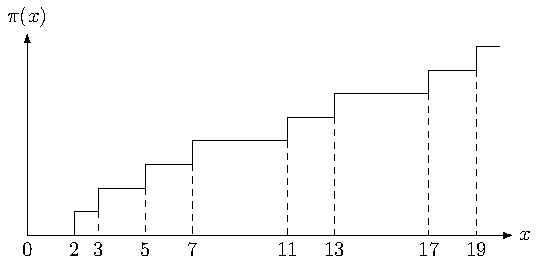
\includegraphics{nkym/fig/pi-x.pdf}
  \caption{素数階段}
  \label{fig:prime-step}
\end{figure}
%
この関数を$\pi(x)$と書く。素数は英語でprime numberというので、その頭文字pに対応するギリシャ文字$\pi$という名前が付けられている。円周率とは関係ない。\par
$\pi(x)$には$x$以下の素数の個数という意味がある。つまり$\pi(x)$を具体的な$x$の式として表すことができれば、素数の分布が正確にわかることになる。果たしてそのようなことができるのであろうか。まずは近似式
  \footnote{
      ここでは近似記号\quotation{$\sim$}(ニョロ)は
      \begin{align*}
        f(x) \sim g(x) \quad (x\to\infty)
        \overset{\text{def}}{\iff} \lim_{x\to\infty} \frac{f(x)}{g(x)} = 1
      \end{align*}
      と定義されているとする。
  }
として、以下の定理を与える。
\begin{thm}{定理(素数公式)}
  $\pi(x)$について、以下の近似式が成り立つ。
  \begin{align}
    \pi(x) \sim \frac{x}{\log x} \sim \li(x)
    \quad (x\to\infty).
  \end{align}
  ここで$\li(x)$は次式で定義される対数積分関数である。
  \begin{align}
    \li(x) := \int_2^x \frac{\dd{u}}{\log u}.
  \end{align}
\end{thm}
%
\begin{remark}
  $x/\log x$より$\li(x)$の方が近似の精度がよいことが示されている。
\end{remark}
%
\begin{prf}
  省略(ToT)
\end{prf}

%
\begin{thm}{定理(明示公式)}
  $\pi(x)$について、以下の等式が成り立つ。
  \begin{align*}
    \pi(x) = \sum_{m=1}^\infty \frac{\mu(m)}{m}
      \qty\bigg(
        \Li(x^\frac1m) - \sum_{\widehat\zeta(\rho)=0} \Li(x^\frac{\rho}m)
        - \log2 + \int_{x^\frac1m}^\infty \frac{\dd{u}}{(u^2-1)u\log{u}}
      ).
  \end{align*}
\end{thm}
%
\begin{remark}
  上の定理において、$\Li(x)$は
  \begin{align*}
    \Li(x) := \int_0^x \frac{\dd{u}}{\log u}
    \equiv \lim_{\epsilon\to +0} \qty(
      \int_0^{1-\epsilon} \frac{\dd{u}}{\log u} + \int_{1+\epsilon}^x \frac{\dd{u}}{\log u}
    )
  \end{align*}
  で定義される対数積分であり、$\rho$は$\zeta(s)$の非自明な零点を表す。
  また、$\mu(m)$はメビウス関数と呼ばれ
  \begin{align*}
    \mu(m) := 
    \begin{cases}
      +1 & \quad \text{\zenkakko{$m$が偶数個の相違なる素数の積}} \\
      -1 & \quad \text{\zenkakko{$m$が奇数個の相違なる素数の積}} \\
      0 & \quad \text{\zenkakko{$m$が素数の平方で割れる}}
    \end{cases}
  \end{align*}
  と定義されている。具体的には
  \begin{table}[H]
    \centering
    \begin{tabular}{c|ccccccccccc}
      $m$      & 1 &  2 &  3 & 4 &  5 & 6 &  7 & 8 & 9 & 10  \\ \hline
      $\mu(m)$ & 1 & $-1$ & $-1$ & 0 & $-1$ & 1 & $-1$ & 0 & 0 & 1
    \end{tabular}
  \end{table}
  のようである。
\end{remark}
%
\begin{prf}
  省略(ToT)
\end{prf}

この定理は$\pi(x)$に厳密に等しい式を与えている。そしてそこにゼータ関数の非自明な零点が絡んでいる!!!! 
しかし、$\pi(x)$の式が与えられたといっても、無限級数や広義積分が使われているため、数値計算で厳密に$\pi(x)$を知ることはできない。さらにゼータ関数の零点も無限個あるのでなおさらだ。こんな式は使わないで、普通に素数判定プログラム作った方が早そう......


% - - - - - - - - - - - - - - - - -
\subsection{リーマン予想とRSA暗号}
% - - - - - - - - - - - - - - - - -
某公共放送局の某番組でそのように伝えられてしまったが故かは知らないが、リーマン予想が証明されるとRSA暗号(現在一般的な暗号方式)が無意味になってしまうなどと、いくらかの人がそういう心配をしているのをたまに見かける。結論から言えばそんなことはない。\par
RSA暗号は、簡単というかテキトーに言うと、デカイ素数の積(公開鍵)をその約数であるデカイ素数(秘密鍵)を用いて因数分解することで暗号を復元している。これがなぜ暗号として機能するかというと、デカイ数の因数分解は短時間(例えば数ヶ月)では計算できないからである。素因数分解のアルゴリズムはいろいろあるが、わざわざそれに前節に書いた$\pi(x)$の公式を使って素数判定するのは賢くない。$\zeta(s)$の非自明な零点が$\Re(s)=\frac12$にしかないということがわかれば、確かに非自明な零点を探すのは楽になるがそれだけである。\par
例え暗号方式などについて全くの無知であっても、リーマン予想が解かれることで現在使われている暗号が無意味になってしまうという主張は正しくないことがわかる。もしリーマン予想が暗号解読に繋がるのならば、仮にそれが真であると仮定してしまえば暗号は解読できることになってしまう。リーマン予想は広く知られているのに、現在もRSA暗号が使われていることから、リーマン予想は暗号解読に影響しないことがわかる。よって、リーマン予想が証明されたところで世の中は大して変わらない。数学界については知らないが。\par
暗号解読に関係するのはむしろ、$\mathrm{P}\ne\mathrm{NP}$予想と呼ばれる問題の方である。こちらもミレニアム懸賞問題になっている。よくわからんが、現在では因数分解を多項式時間で行うアルゴリズムは見つかっていないが、もし$\mathrm{P}=\mathrm{NP}$が証明されてしまうと、多項式時間で因数分解ができるアルゴリズムが存在することになってしまうらしい。そしてもしそのアルゴリズムが発見されると、今度こそRSA暗号が簡単に解読することができてしまうのかな? ただし、$\mathrm{P}\ne\mathrm{NP}$予想という名前からわかるように、$\mathrm{P}\ne\mathrm{NP}$であるだろうと多くの人が考えているらしい。



% - - - - - - - - - - - - - - - - - - - - - - - -
\subsection{数値計算(ギャラリー)}
% - - - - - - - - - - - - - - - - - - - - - - - -
最後に付録として、$\Gamma(s)$や$\zeta(s)$、素数公式の様子などをFortranで数値計算し、GnuplotとTi$k$Zを用いて
\footnote{
  Gnuplotでpdfを直接出力しても十分美しいグラフを作成できるが、Gnuplotの出力先をTi$k$Zに変更し(\verb|set terminal tikz|)、\LaTeX を経由してグラフを作成した方がより美しいものが得られる。その際には、\LaTeX 側でプリアンブルに\verb|\usepackage{gnuplot-lua-tikz}|と記し、\verb|\input|コマンドでGnuplotが吐いたtexファイルを読み込むだけでよい。ただし、Gnuplotからgnuplot-lua-tikz.styを生成しておく必要がある。
  }
美しい\zenkakko{?}図を作成したので、それらをいくつか載せておく。
クリティカルライン$\Re(s)=\frac12$上の$\zeta(s)$も計算したので是非参照されたい。


%
\subsubsection{ガンマ関数$\Gamma(s)$}
%
まずは、相反公式を変形した
\begin{align}
  \Gamma(s) = \frac{\pi}{\Gamma(1-s) \sin \pi s}
  \label{eq:gamma-setuzoku-sohan}
\end{align}
によって複素数全体へと解析接続されたガンマ関数$\Gamma(s)$のグラフを紹介する。ガンマ関数の性質
\begin{align}
  \Gamma(s+1) = s\Gamma(s)
  \label{eq:Gamma-1}
\end{align}
を用いて計算するより、(\ref{eq:gamma-setuzoku-sohan})を用いた方が多少精度が良かった。とはいえ、図\ref{fig:gamma-real}を見ればわかりやすいが、$s$が$-4$より小さいところでは無限大に発散する様子が上手く描かれていない。教科書に載っているような美しい図を描くのはなかなか難しそうである。
素人のプログラムではこれが限界だったので堪忍していただきたい。

%
\begin{figure}[H]
  \centering
  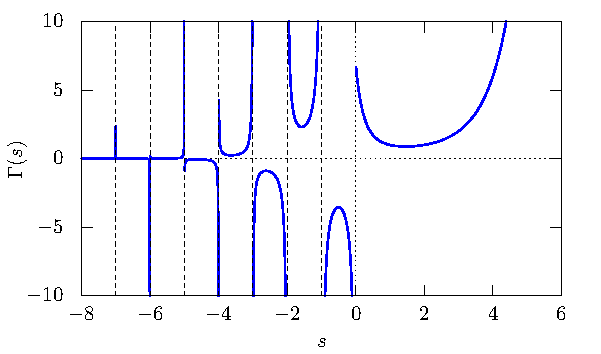
\includegraphics{nkym/gnuplot/gamma/real-main.pdf}
  \caption{解析接続した$\Gamma(s)$。$s$および$\Gamma(s)$は実数。}
  \label{fig:gamma-real}
\end{figure}

図\ref{fig:gamma-complex}は$x,y$軸に引数$s$の実部と虚部を表し、$z$軸に$\Gamma(s)$の絶対値を表している。虚軸付近に小さな山が見えるが、これは計算精度のせいで生じてしまったものであり、実際は存在しないらしい。ガンマ関数を数値計算するときはLanczos近似というものを使うのが良いらしいが、ここでは深入りしない。
%
\begin{figure}[H]
  \centering
  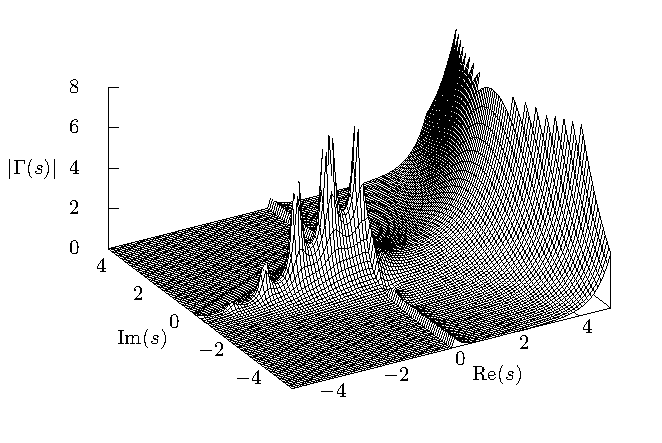
\includegraphics{nkym/gnuplot/gamma/complex-main.pdf}
  \caption{$|\Gamma(s)|$の値。3次元プロット。}
  \label{fig:gamma-complex}
\end{figure}

% \clearpage
%
\subsubsection{素数階段と素数公式}
次に、素数公式
\begin{align}
  \pi(x) \sim \frac{x}{\log x} \sim \li(x)
  \quad (x\to\infty)
\end{align}
の様子を図にした。図\ref{fig:prime-step100},\ref{fig:prime-step500}を見ると、確かに素数公式は正しいようであることがわかる。
また、$x$がある程度大きいところでは、常に$x/\log x < \pi(x) < \li(x)$の関係があることがわかる。\par
明示公式の方については、式を見るだけで非常に面倒臭いことを悟ってしまったので、今回はパスすることにした。tsujimotterさん
\footnote{\url{http://tsujimotter.hatenablog.com/about}}
が明示公式が$\pi(x)$に収束する様子を体感できるブラウザアプリを公開していたので、是非そちら
\footnote{こちら:「リーマンの素数公式を可視化する」\url{http://tsujimotter.hatenablog.com/entry/2014/06/29/002109}}
で確認していただきたい。

%
\begin{figure}[p]
  \centering
  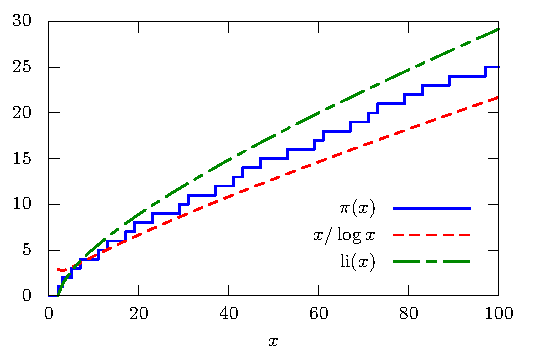
\includegraphics{nkym/gnuplot/prime-step/100main.pdf}
  \caption{$\pi(x)$とその近似式。$x\le100$。}
  \label{fig:prime-step100}
\end{figure}
%
\begin{figure}[p]
  \centering
  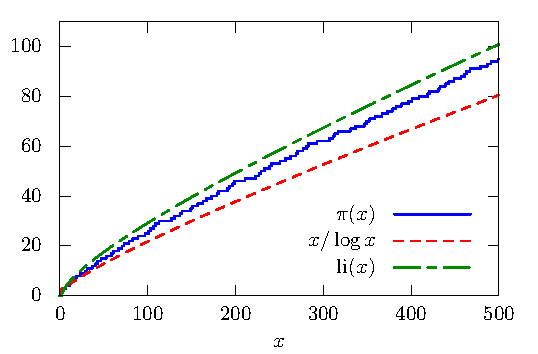
\includegraphics{nkym/gnuplot/prime-step/500main.pdf}
  \caption{$\pi(x)$とその近似式。$x\le500$。}
  \label{fig:prime-step500}
\end{figure}

\clearpage

%
\subsubsection{ゼータ関数$\zeta(s)$}
初めに$s>1$について級数で定義したゼータ関数(\ref{eq:zeta})の様子を見てみる。当然無限回足しあげるのは不可能なので、第$N$項までで切り上げることにする。
\begin{align*}
  \zeta(s) = \sum_{n=1}^N\frac1{n^s}.
\end{align*}
図\ref{fig:lt1-zeta}を見ればわかるように、この級数は収束が非常に遅い。$s\to1$で$\zeta(s)\to\infty$になることは既に示したが、図\ref{fig:lt1-zeta}で見られるように、$N=10^6=1,000,000$まで足し上げても$s\to1$で$\zeta(s)$は$14$にも満たない。
%
\begin{figure}[H]
  \centering
  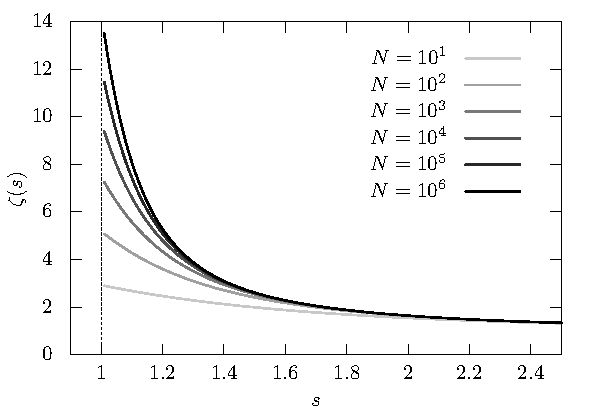
\includegraphics{nkym/gnuplot/zeta/lt1-main}
  \caption{級数表示(\ref{eq:zeta})による$\zeta(s)$。}
  \label{fig:lt1-zeta}
\end{figure}
%
\ref{sec:zeta}節の(\ref{eq:zeta-s>0})で$\zeta(s)$を解析接続した際にも、$s= 1+\varepsilon$における収束性の悪さが、$\Re(s)$が1以下の領域にも影響してくる。実際、この解析接続で$\zeta(s)$の値を計算してみたが、やはり上手くいかなかった。\par
そこで、本文中では証明を与えていないが、tsujimotterさん
などいくつかのサイトで紹介されている次の式で$\zeta(s)$を$s=1$を除く複素数全体へ解析接続する。
\begin{align}
  \zeta(s) &:= \frac{1}{1 - 2^{1-s}} \sum_{m=1}^\infty 2^{-m} \sum_{j=1}^m (-1)^{j-1} \binom{m-1}{j-1}j^{-s}.
  \label{eq:zeta-tsujimoter}
\end{align}
この解析接続の証明はせきゅーんさん
\footnote{http://integers.hatenablog.com/about}
の記事「リーマンゼータ関数の級数表示による解析接続(\url{http://integers.hatenablog.com/entry/2016/08/16/133319})」で紹介されている。
今回はこの式を使わせていただいて、$\zeta(s)$の数値計算をしてみようと思う。\par
まずは実軸上の値を計算し、$s>1$ではちゃんと解析接続する前の$\zeta(s)$と一致していることを確認する。
%
\begin{figure}[H]
  \centering
  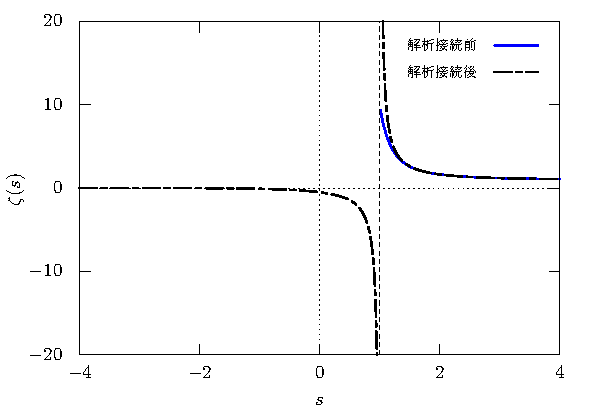
\includegraphics{nkym/gnuplot/zeta02/real-main.pdf}
  \caption{解析接続した$\zeta(s)$。$s$は実数。}
  \label{fig:real-zeta}
\end{figure}
%
図\ref{fig:real-zeta}からわかるように、(\ref{eq:zeta-tsujimoter})で解析接続した$\zeta(s)$は$s>1$でちゃんと解析接続前と一致するどころか、解析接続前のものより収束が速くなっている。この図を描くとき外側の級数は$m=10$までしか足し上げていない。それでこんなに収束が速くなるので驚きだ。\par
この式を信用してもらえたところで、次は実軸上の自明な零点について見てみる。$s<0$での振動は非常に小さく、図\ref{fig:real-zeta}では零点があるのかよくわからいのでもう少し拡大してみる。
%
\begin{figure}[H]
  \centering
  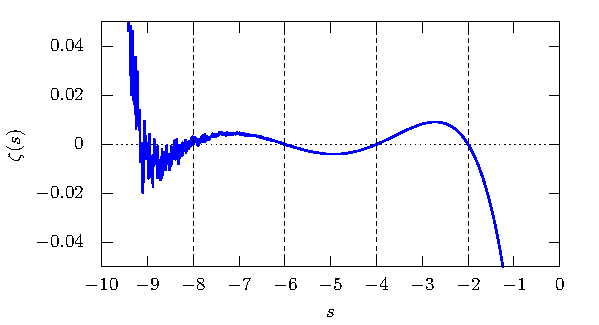
\includegraphics{nkym/gnuplot/zeta02/jimei-main.pdf}
  \caption{解析接続した$\zeta(s)$の自明な零点。}
  \label{fig:jimei-zeta}
\end{figure}
%
図\ref{fig:jimei-zeta}から確かに$\zeta(s)$は$s$が負の偶数に零点を持っていることがわかる。しかし私のチーププログラムでは$s=-8$ぐらいまでが限界で、それより小さいところの様子はわからない。こちらも$\zeta(s)$の値を計算するとき外側の級数は$m=10$までにしてある。$m$の上限をあげると精度が増すはずなのだが、あまりそれをしてしまうと二項係数の部分がオーバーフローしてしまい、訳のわからないことになってしまう(これで5時間ほど無駄にした)。とりあえず自明な零点についてはこれで妥協していただきたい。\par
%
\begin{figure}[H]
  \centering
  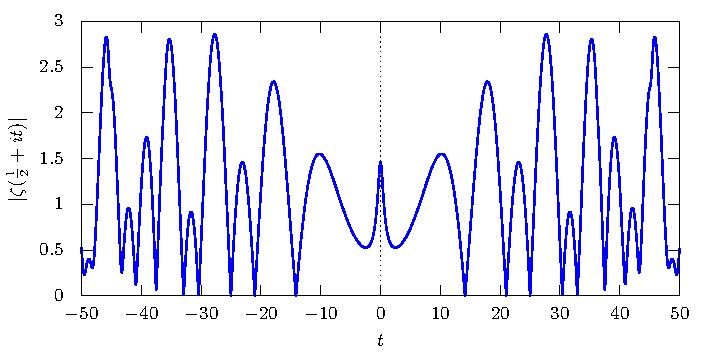
\includegraphics{nkym/gnuplot/zeta02/hijimei-main.pdf}
  \caption{解析接続した$\zeta(s)$の非自明な零点。}
  \label{fig:hijimei-zeta}
\end{figure}
%

\clearpage

次に本題である$\zeta(s)$の非自明な零点について見てみる(図\ref{fig:hijimei-zeta})。リーマンによって$\zeta(s)$の非自明な零点は全て$s=\frac12+it$上にあるだろうと予想されている。この直線はクリティカルラインと呼ばれている。\par
複素変数の複素関数を2次元や3次元にプロットするのは困難なので、以降$\zeta(s)$の値は絶対値を取ることにする。図\ref{fig:hijimei-zeta}が左右対称になっているのはそのためである
\footnote{
  一般に複素数$z$について、実数$x,y$を用いて$z=x+iy$と書けたとすると、$|z|\equiv\sqrt{\bar{z}z}$であるから、
  $|\bar{z}| = \sqrt{\bar{\bar{z}}\bar{z}} = \sqrt{z\bar{z}} = \sqrt{\bar{z}z}$となり、
  $|z|=|\bar{z}|$すなわち$|x+iy|=|x-iy|$であるので、複素数の絶対値は虚部について反転対称性がある。
}。\par
先人たちによって既に知られている非自明な零点の虚部を、原点に近い順に書いてみると、以下の表のようである
\footnote{引用元:\url{http://www.lmfdb.org/zeros/zeta/}}
。ただし虚部が負の部分は省略している。
%
\begin{table}[H]
  \small
  \centering
  \caption{$\zeta(s)$の非自明な零点}
  \label{tb:hijimei-zeta}
  \begin{tabular}{rl}\hline
    番号 & 虚部$\Im(s)=t$\\ \hline
    1 & 14.1347251417346937904572519835624766\\
    2 & 21.0220396387715549926284795938969162\\
    3 & 25.0108575801456887632137909925627734\\
    4 & 30.4248761258595132103118975305839571\\
    5 & 32.9350615877391896906623689640747418\\
    6 & 37.5861781588256712572177634807052984\\
    7 & 40.9187190121474951873981269146334247\\
    8 & 43.3270732809149995194961221654068456\\
    9 & 48.0051508811671597279424727494276636\\
    10 & 49.7738324776723021819167846785638367 \\ \hline
  \end{tabular}
\end{table}
%
表\ref{tb:hijimei-zeta}を参照しつつ図\ref{fig:hijimei-zeta}を見てみると、確かに$t=14,21,25,30,33$付近に零点があることがわかる。\par
最後に$\zeta(s)$の3次元プロットを見て終わりにしよう。
図\ref{fig:complex-zeta}は原点周りの$\zeta(s)$の全体像である。1つ目の非自明な零点が見られる。\par
また、図\ref{fig:3d-jimei-zeta}は実軸付近の様子を描いている。
自明な零点と$s=1$で発散する点が見られる。ただし自明な零点の凹凸は非常に小さいため、$|\zeta(s)|$の値は対数表示している。

\clearpage

%
\begin{figure}[p]
  \centering
  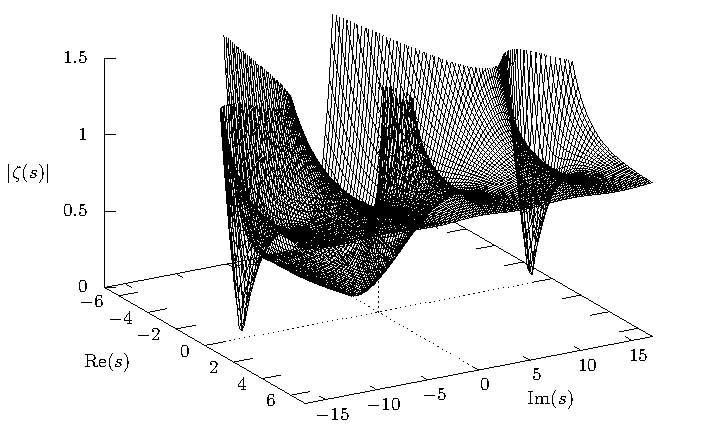
\includegraphics{nkym/gnuplot/zeta03/complex-main.pdf}
  \caption{$|\zeta(s)|$の値。3次元プロット。}
  \label{fig:complex-zeta}
\end{figure}
%

%
\begin{figure}[p]
  \centering
  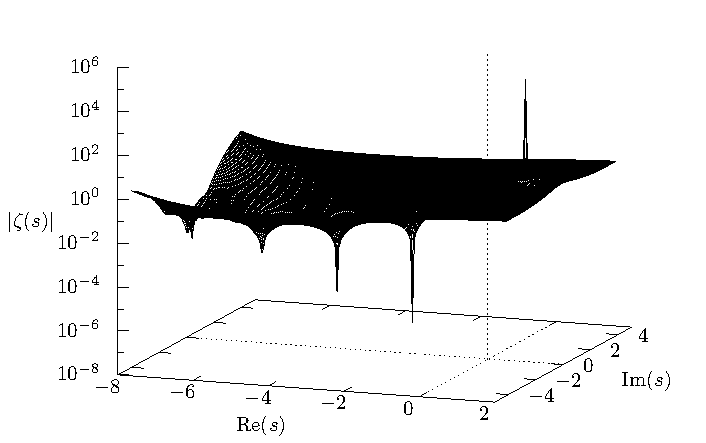
\includegraphics{nkym/gnuplot/zeta03/jimei-main.pdf}
  \caption{実軸付近。$|\zeta(s)|$の自明な零点が見られる。}
  \label{fig:3d-jimei-zeta}
\end{figure}
%

\clearpage

図\ref{fig:3d-hijimei-zeta}はクリティカルライン$s=\frac12+it$付近の$|\zeta(s)|$の値を描いている。一体どういう規則で非自明な零点は現れるのであろうか。
%
\begin{figure}[H]
  \centering
  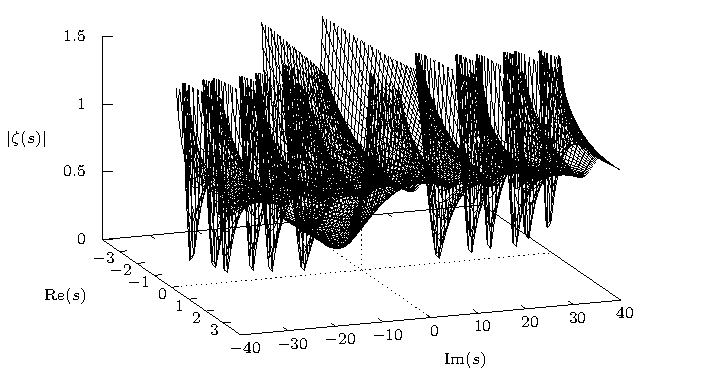
\includegraphics{nkym/gnuplot/zeta03/hijimei-main.pdf}
  \caption{クリティカルライン付近。$|\zeta(s)|$の非自明な零点が見られる。}
  \label{fig:3d-hijimei-zeta}
\end{figure}


%               T H E  E N D

%  T H A N K  Y O U  F O R  R E A D I N G




% - - - - - - - - - - - - - - - - -
\end{document}

% EOF
